% Copyright (C)  2016 Philipp Hacker.
% Permission is granted to copy, distribute and/or modify this document
% under the terms of the GNU Free Documentation License, Version 1.3
% or any later version published by the Free Software Foundation;
% with no Invariant Sections, no Front-Cover Texts, and no Back-Cover Texts.
% The lincense itself can be found at <https://www.gnu.org/licenses/fdl-1.3>.

\documentclass[a4paper,10pt]{article}
%\documentclass[numbers=noenddot,12pt,a4paper,notitlepage,twoside,BCOR15mm]{scrartcl}

\usepackage{lipsum}
\usepackage{multicol}

\usepackage[T1]{fontenc}
\usepackage[utf8]{inputenc}

\usepackage[infoshow]{tabularx}
\usepackage[all]{xy}

\usepackage{geometry}
\geometry{%
	a4paper,
	left=24mm,
	right=24mm,
	top=24mm,
	bottom=24mm,
	}

\usepackage{amsmath,mathtools}
\usepackage{amssymb}
\usepackage{units}
\usepackage{upgreek}
\usepackage{esint}
\usepackage{graphicx}
\usepackage{ziffer}

\usepackage{float}
\usepackage{lscape}

\usepackage[labelfont=bf]{caption}
\usepackage{wrapfig}
\usepackage{subcaption}

\usepackage[backref=page]{hyperref}

\usepackage{csquotes}
\usepackage[infoshow]{tabularx}
\usepackage{fancyhdr}

\usepackage{sectsty}
\usepackage{times}

\usepackage{lmodern} %TODO Schriftart
\usepackage[greek,english]{babel} %TODO Sprache einstellen

\renewcommand{\headrulewidth}{0.1pt}
\renewcommand{\footrulewidth}{0.1pt}
\newcommand{\name}{\text{Philipp Hacker}} %TODO Name des Protokollanten eintragen

\setlength{\parindent}{0pt}

\newcommand{\degree}{^\circ}
\newcommand{\diff}{\textnormal{d}}
\newcommand{\tenpo}[1]{ 10^{#1}}
\newcommand{\greek}[1]{\greektext#1\latintext}
\newcommand{\ix}[1]{_\text{#1}}
\newcommand{\imag}{\mathbf{i}}
\newcommand{\tilt}[1]{\textit{#1}}
\newcommand{\grad}[1]{\textit{grad}\left(#1\right)}
\newcommand{\divergenz}[1]{\textit{div}\left(#1\right)}
\newcommand{\euler}{\mathnormal{e}}
\newcommand{\fett}[1]{\textbf{#1}}
\newcommand{\ket}[1]{|#1\rangle}
\newcommand{\bra}[1]{\langle#1|}

\newcommand{\HRule}{\rule{\linewidth}{0.5mm}} % New command to make the lines in the title page

\author{Philipp Hacker} % Your name, this is used in the title page and abstract, print it elsewhere with \author

\newcommand{\prof}{Prof. Dr. Meichsner}

\newcommand{\supname}{Dr. S. Nemschokmichal, R. Tschiersch} % Your supervisor's name, this is used in the title page, print it elsewhere with \supname

\newcommand{\univname}{Ernst-Moritz-Arndt University Greifswald} % Your university's name and URL, this is used in the title page and abstract, print it elsewhere with \univname

\newcommand{\deptname}{Institute of Physics} % Your department's name and URL, this is used in the title page and abstract, print it elsewhere with \deptname

\newcommand{\groupname}{Low-temperature Plasma Physics group} % Your research group's name and URL, this is used in the title page, print it elsewhere with \groupname

\newcommand{\rtitle}{Electric field strength spectroscopy in dielectric barrier discharges}

\date{\today}

\pagestyle{fancy}
\fancyhead[R,L,C]{}
\fancyfoot[R,L,C]{}
\fancyhead[RE]{\href{http://www.physik.uni-greifswald.de/}{\deptname}}
\fancyhead[LO]{\href{http://www1.physik.uni-greifswald.de/}{\groupname}}
\fancyhead[LE]{\today}
\fancyfoot[LO, RE]{\thepage}
\fancyfoot[LE, RO]{Section \thesection}

\begin{document}

	\setcounter{section}{-1}
	
	\renewcommand*{\contentsname}{Table of Contents}
	\renewcommand*{\equationautorefname}{eq.}
	\renewcommand*{\figureautorefname}{fig.}
	\renewcommand*{\tableautorefname}{tab.}
	\renewcommand*{\sectionautorefname}{sec.}
	\renewcommand*{\subsectionautorefname}{subsec.}
	\renewcommand*{\subsubsectionautorefname}{subsec.}
	\renewcommand*{\figurename}{Fig. }
	\renewcommand*{\tablename}{Tab. }

	\renewcommand*{\figurename}{Figure }
	\renewcommand*{\tablename}{Tabel }

	
	\thispagestyle{empty}
	
	\begin{center}
			
			\HRule \\[0.4cm] % Horizontal line
			\huge \fett{\rtitle} \\ % Thesis title
			\HRule \\[.6cm] % Horizontal line
			
			\large \href{http://www.university-url.com}{\univname}

	\begin{figure}[h]
		\centering
		
		\begin{minipage}[t]{0.48\textwidth}
			\begin{center}
			\emph{Author}: \href{https://github.com/RayleighsJeans/ag_praktikum_2016}{\name} \\ %TODO author
			\emph{Examiner:} \prof
			\end{center}
		\end{minipage}
		\hfill
		\begin{minipage}[t]{0.48\textwidth}
			\begin{center}
				\emph{Supervisor}: Dr. S. Nemschokmichal,\\R. Tschiersch \\ %TODO name of supervisor
			\end{center}
		\end{minipage}
	\end{figure}

		\large \textit{Report for an internship at the \groupname of Prof. Dr. Meichsner, submitted in fulfillment of the requirements for the degree}\\[0.1cm] \fett{Master of Science}\\[0.2cm] %TODO UNIVERSITY TEXT
		\textit{in the}\\[0.2cm]
		\href{http://www1.physik.uni-greifswald.de}{\groupname} \\[0.15cm] \href{http://www.physik.uni-greifswald.de}{\deptname} \\[0.3cm] %TODO RESEARCH GROUP/DEPARTMENT

	\end{center}
	
		\vspace{1cm}
	
	\begin{multicols}{2}
		\tableofcontents
	\end{multicols}
	
		\vspace{1cm}
	
		\section{Abstract}
		
	\twocolumn

	\section{Introduction}
	
		\subsection{Dielectric barrier discharges}
		
		\subsection{Temporal development of the electric field stregnth}

	\section{Experimentel set up}
	
		\subsection{Discharge configurations}
		
		\subsection{Optical emission spectroscopy}

	\section{Results}

		\subsection{Integrated spectrum}
		
			Text.
		
				\begin{figure}[h]
					\centering
					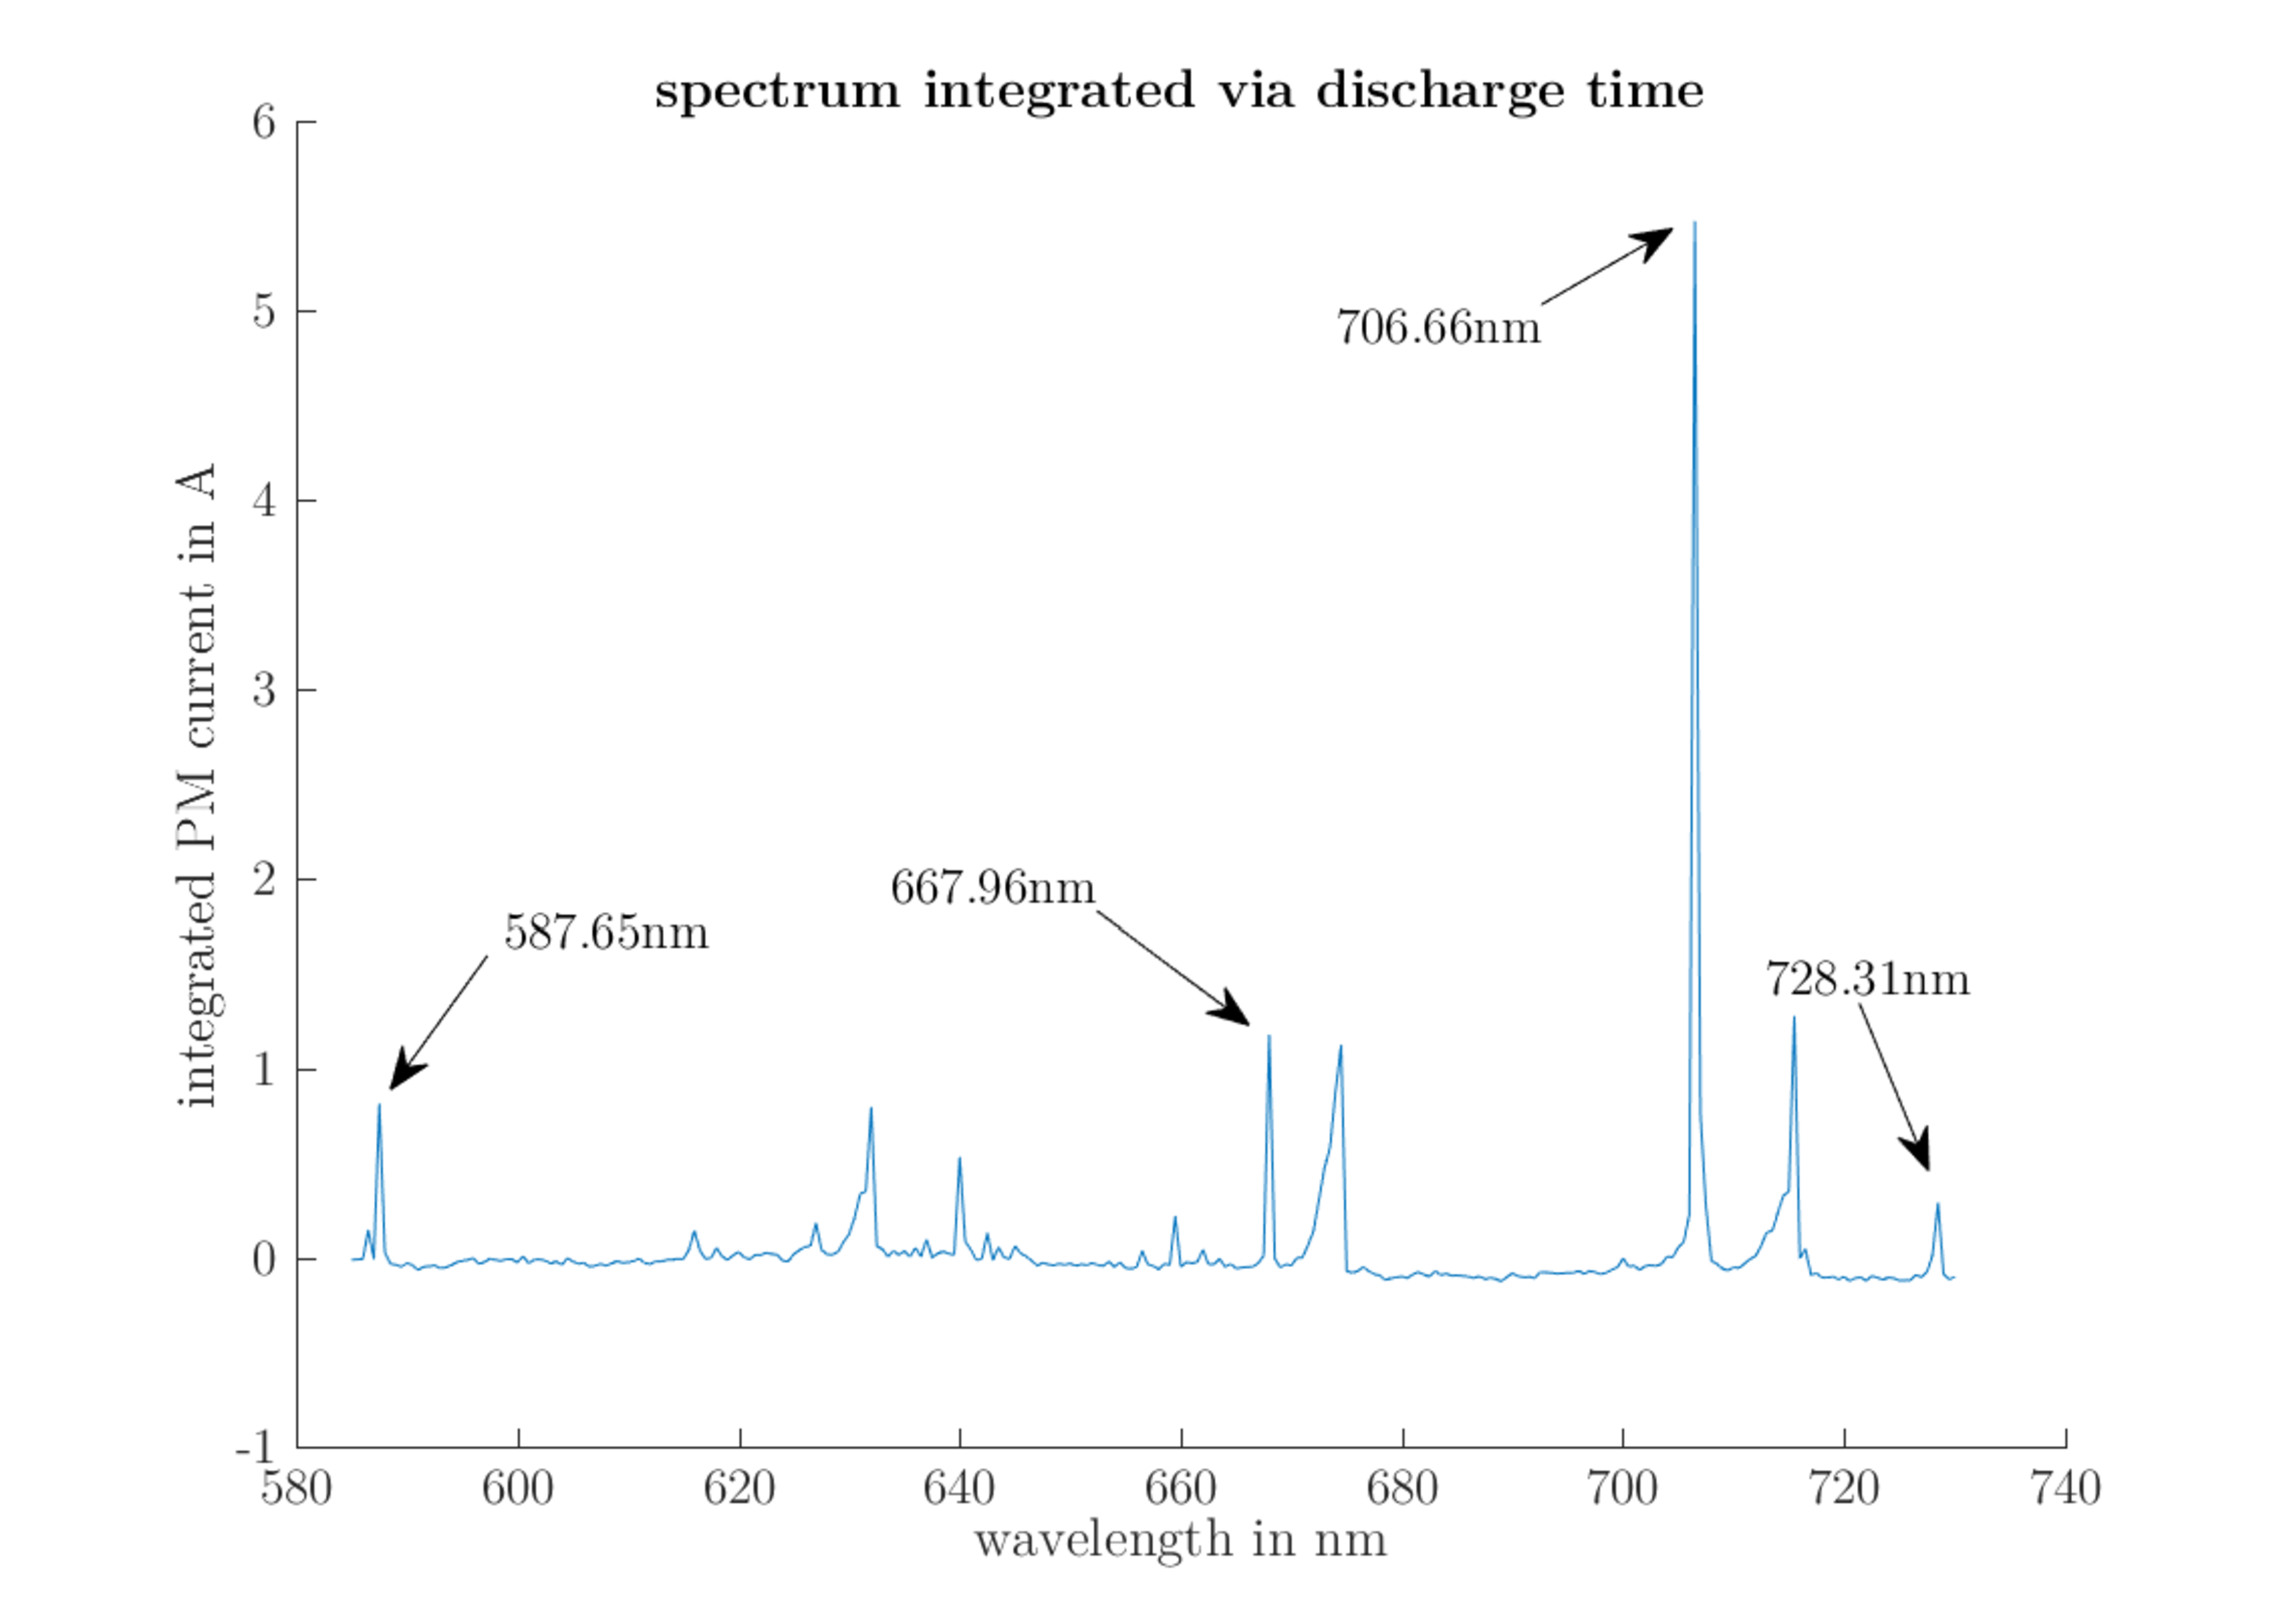
\includegraphics[width=0.5\textwidth]{figures/results/spectrum/int_spectrum.pdf}
					\caption{Integrated photomultiplier current via discharge time. Indicated are the majoring peaks, which will be target of our investigation. The spectrum reaches from $\unit[580]{nm}$ to $\unit[730]{nm}$.}
					\label{img:int_spectrum}
				\end{figure}
				
			Text.
				
				\begin{figure}[h]
					\centering
					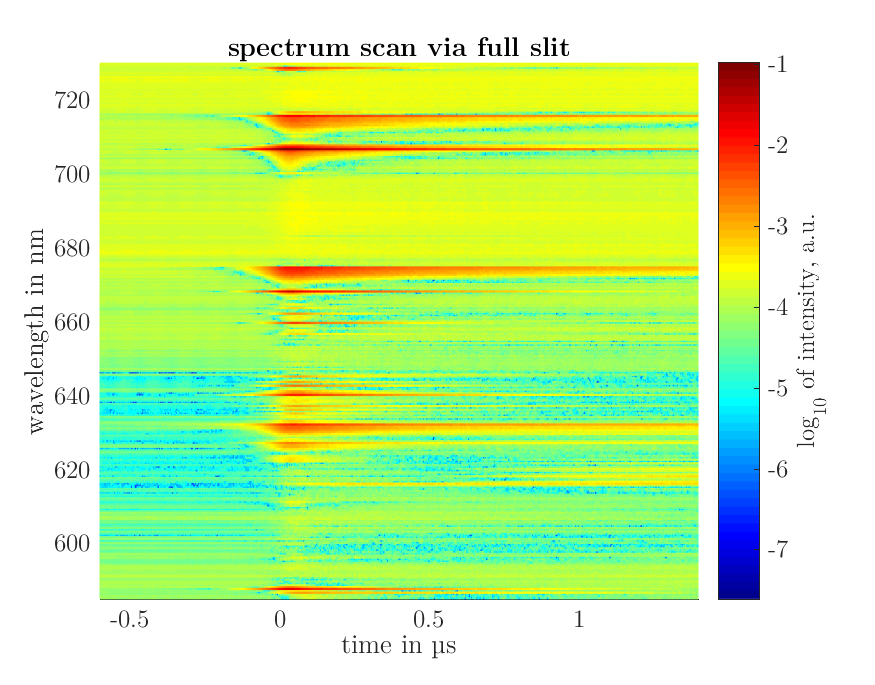
\includegraphics[width=0.5\textwidth]{figures/results/spectrum/spectrum.pdf}
					\caption{Photomultiplier current via discharge time and wavelength. The current derrives from the intensity of the full exit slit of the discharge chamber.}
					\label{img:full_spectrum}
				\end{figure}
				
			Text.
		
		\subsection{Spatial temporal resolved intensities}
		
			Text.
			
		\onecolumn
					
				\begin{figure}[h]
					
					\centering
					
					\begin{subfigure}[t]{0.49\textwidth}
						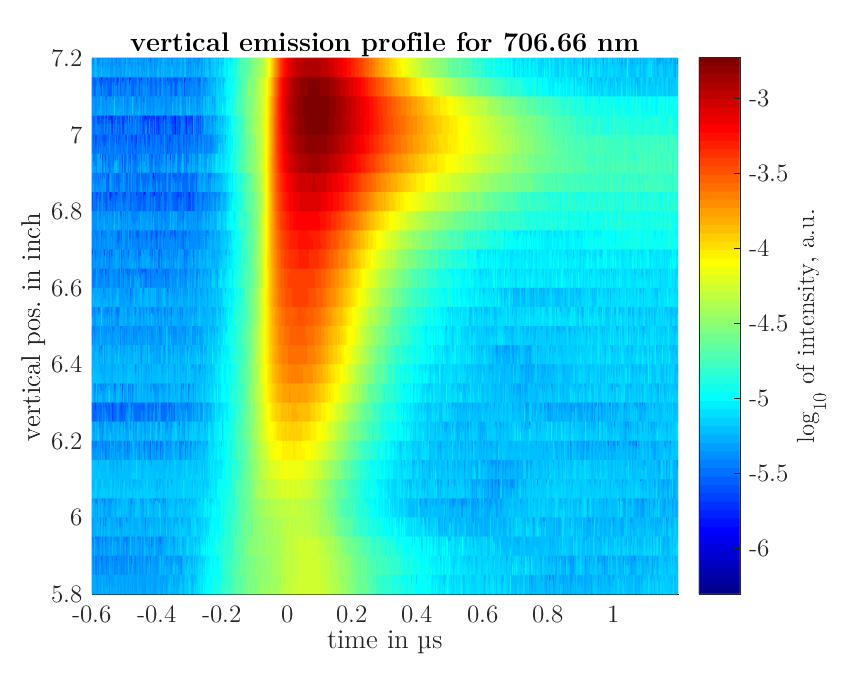
\includegraphics[width=\textwidth]{figures/results/spatialtemporalresolvedlineintensity/sine/706nm.pdf}
						\label{img:706sine}
					     \vspace{-0.5cm}\caption{}
					\end{subfigure}
					\hfill
					\begin{subfigure}[t]{0.49\textwidth}
						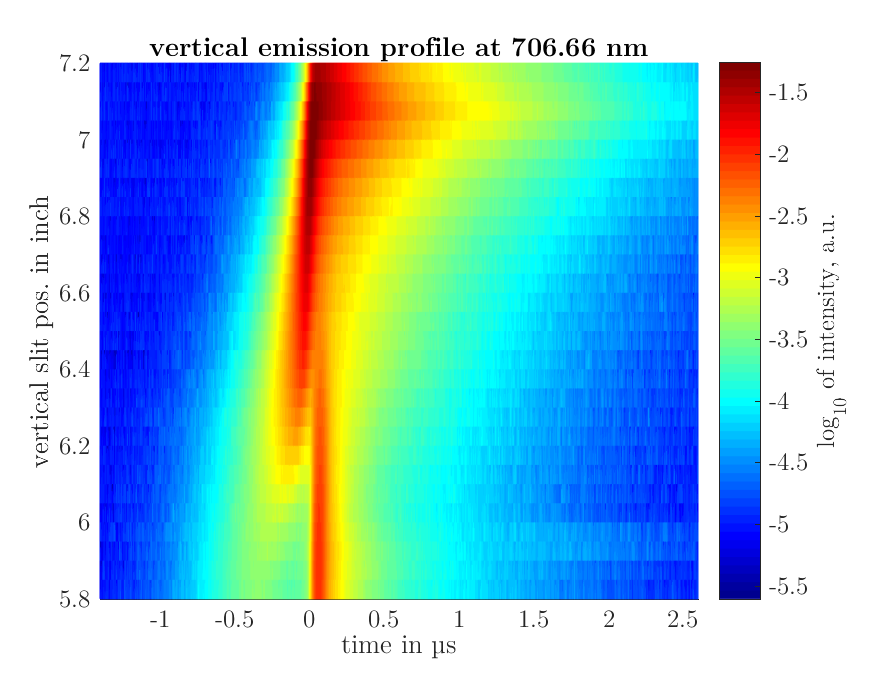
\includegraphics[width=\textwidth]{figures/results/spatialtemporalresolvedlineintensity/square/korr706nm.pdf}
						\label{img:706square}
						\vspace{-0.5cm}\caption{}
					\end{subfigure}
					
					\begin{subfigure}[b]{0.49\textwidth}
						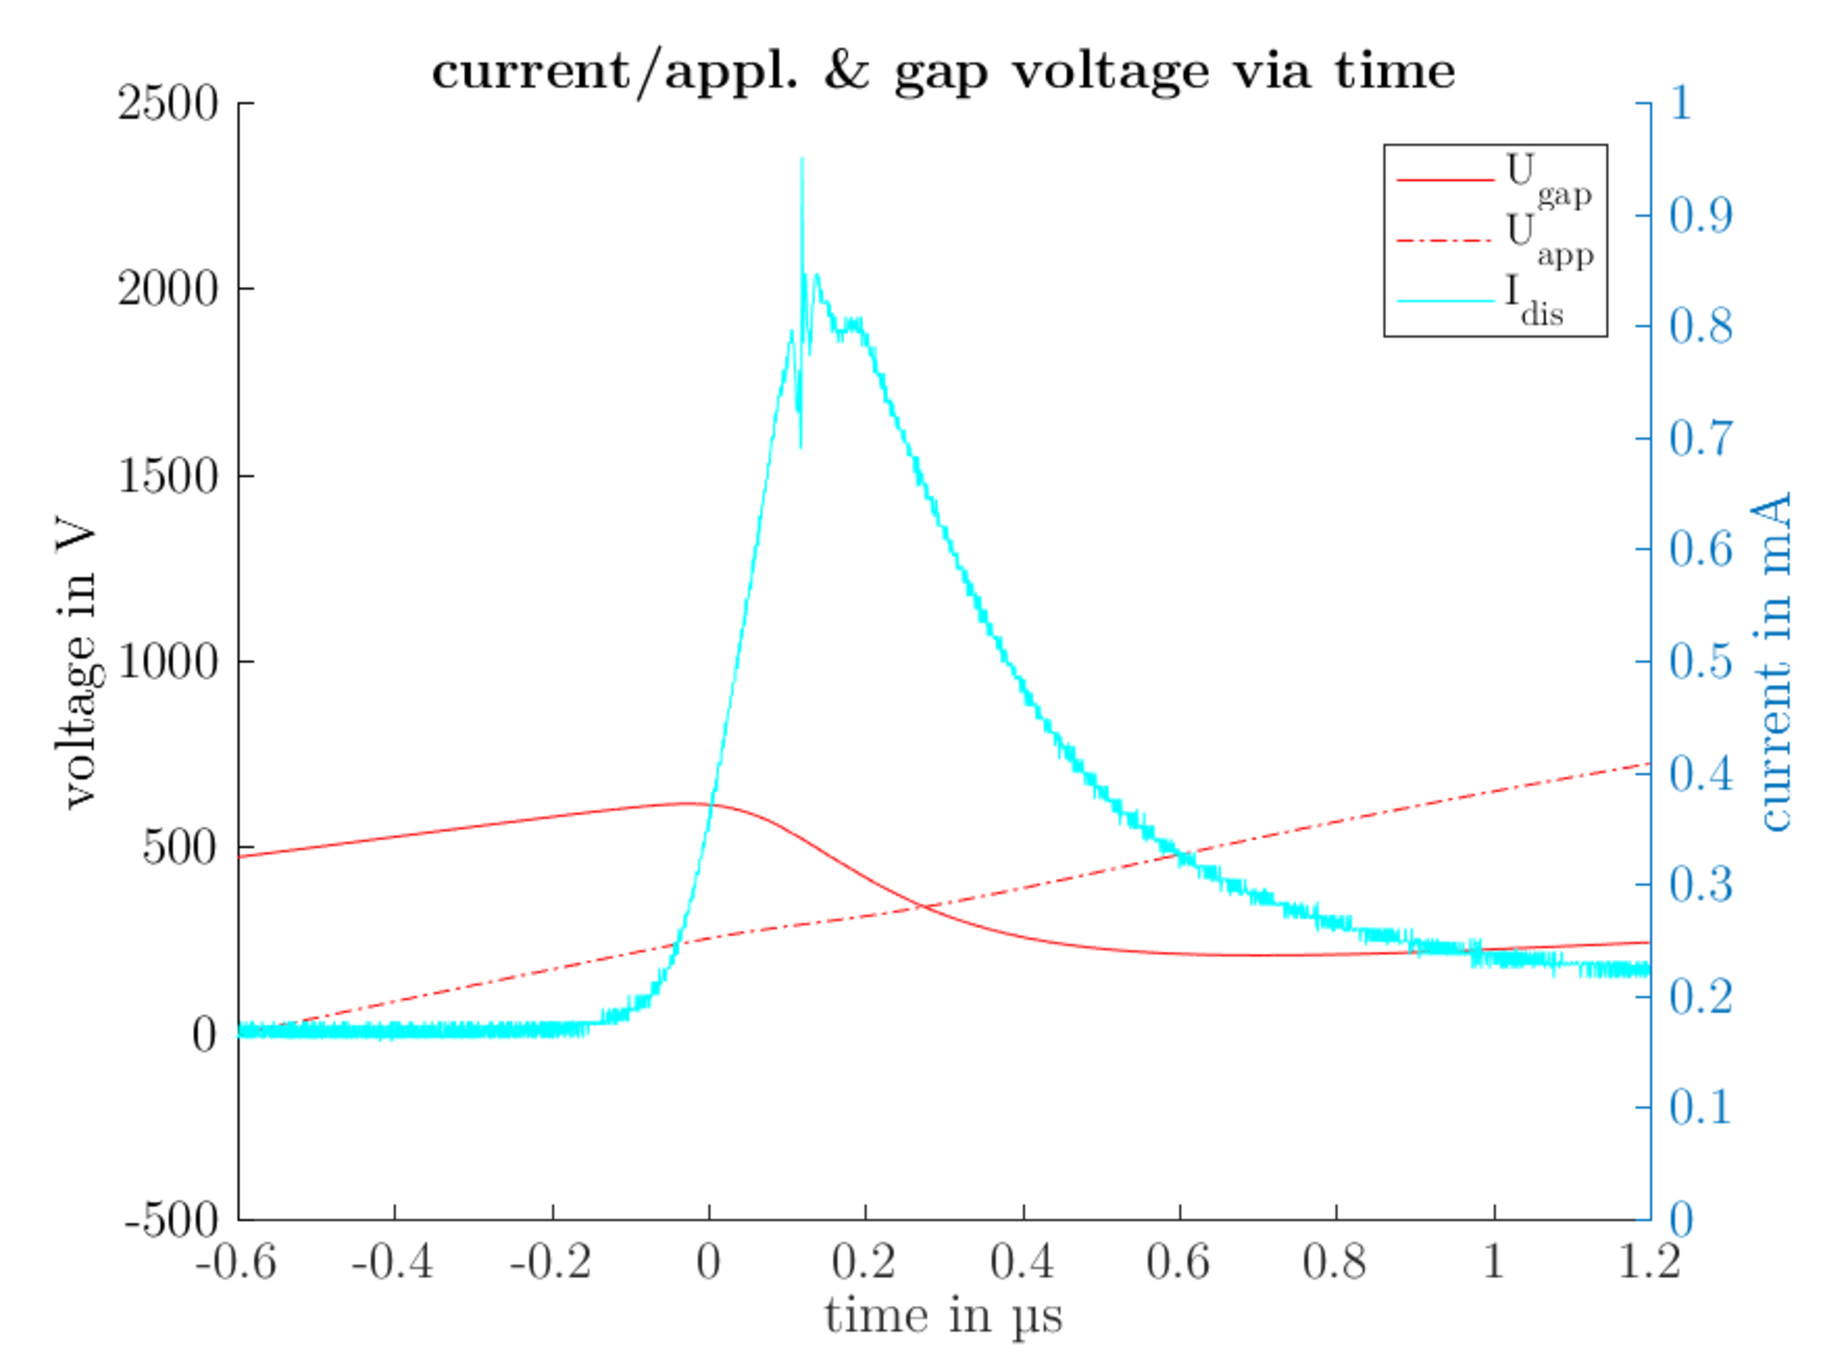
\includegraphics[width=\textwidth]{figures/results/spatialtemporalresolvedlineintensity/sine/current_dis.pdf}
						\label{img:currentdissine}
						\vspace{-0.5cm}\caption{}
					\end{subfigure}
					\hfill
					\begin{subfigure}[b]{0.49\textwidth}
						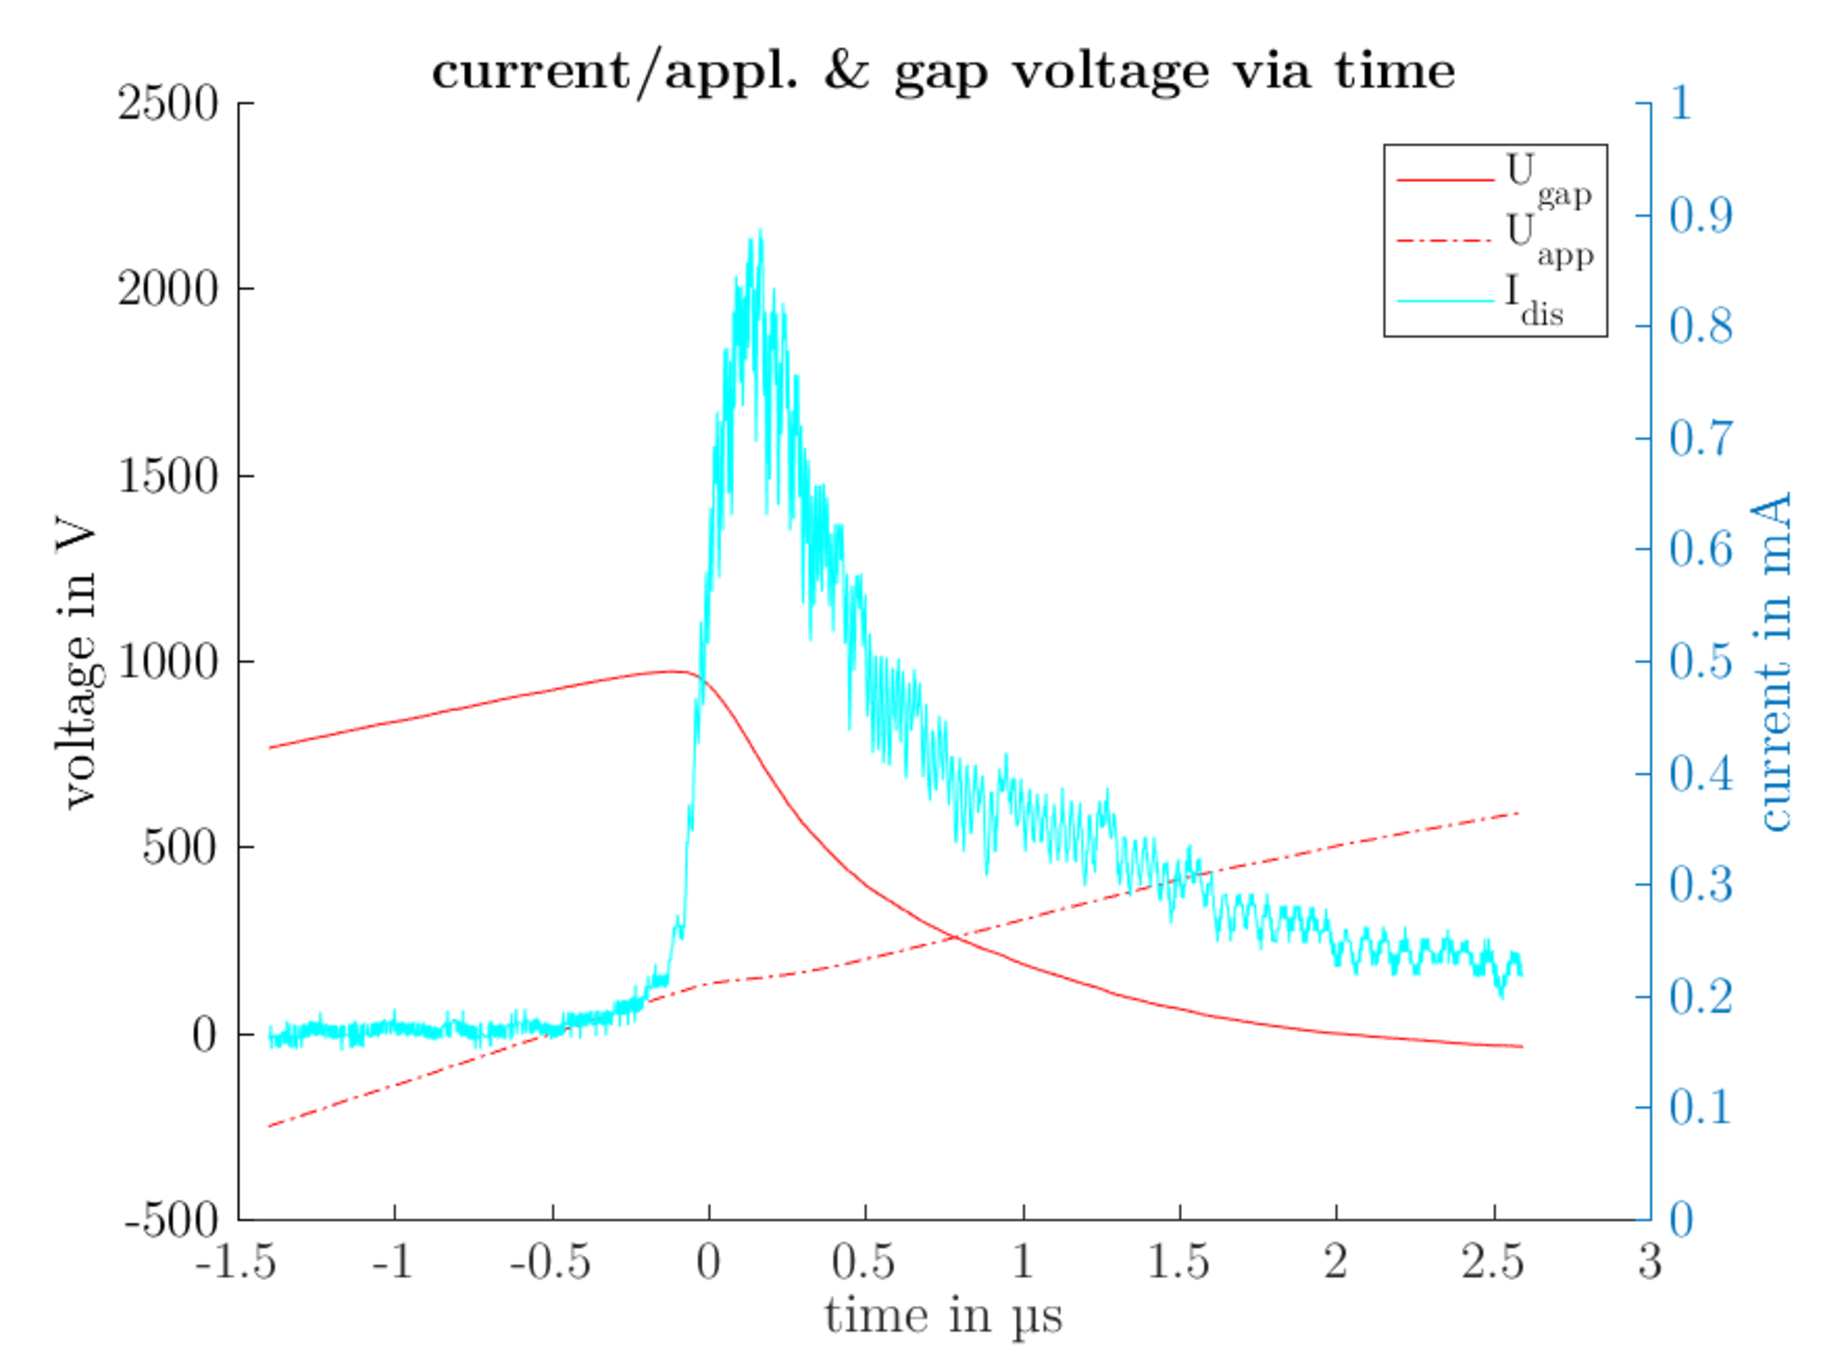
\includegraphics[width=\textwidth]{figures/results/spatialtemporalresolvedlineintensity/square/current_dis.pdf}
						\label{img:currentdissquare}
						\vspace{-0.5cm}\caption{}
					\end{subfigure}
					
					\caption{\fett{(a):} Spatial temporal resolved line emission from $\unit[706.66]{nm}$ at sine wave discharge duty form. \fett{(b):} Profile at square wave duty form. \fett{(c):} Discharge current, gap and applied voltage via time. The graph of the applied voltage resembles a temporal highly resoluted sine wave of $\unit[5]{kHz}$. \fett{(d):} Discharge characteristics for a square wave.}
				\end{figure}
				
		\twocolumn
		
		\subsection{Line ratios}

		\onecolumn
		
				\begin{figure}
					\centering
			
					\begin{subfigure}[t]{0.48\textwidth}
						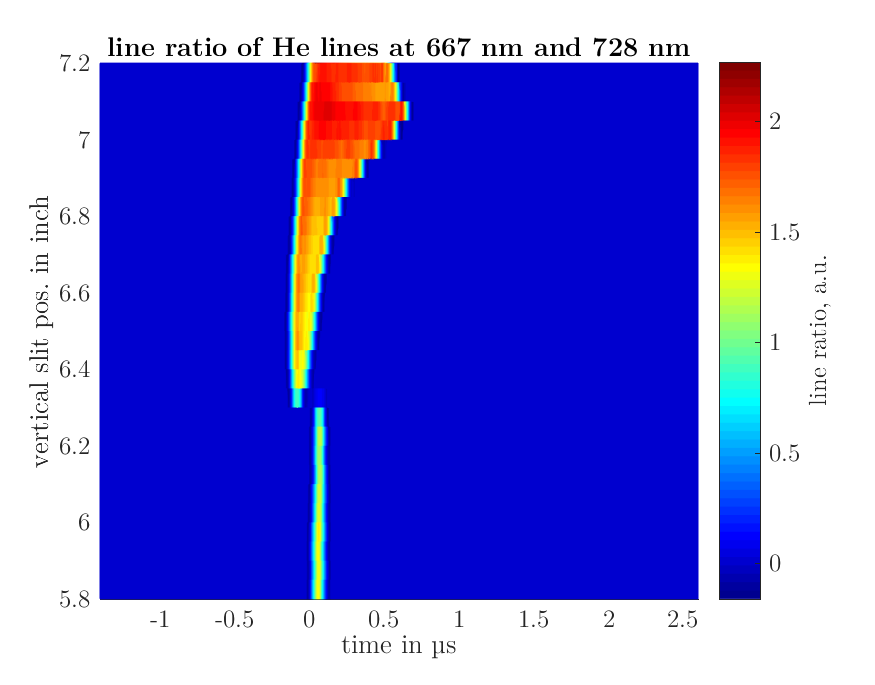
\includegraphics[width=\textwidth]{figures/results/lineratios/square/lineratio667}
						\vspace{-0.5cm}\caption{}
						\label{img:ratio667}
					\end{subfigure}
					\hfill
					\begin{subfigure}[t]{0.48\textwidth}
						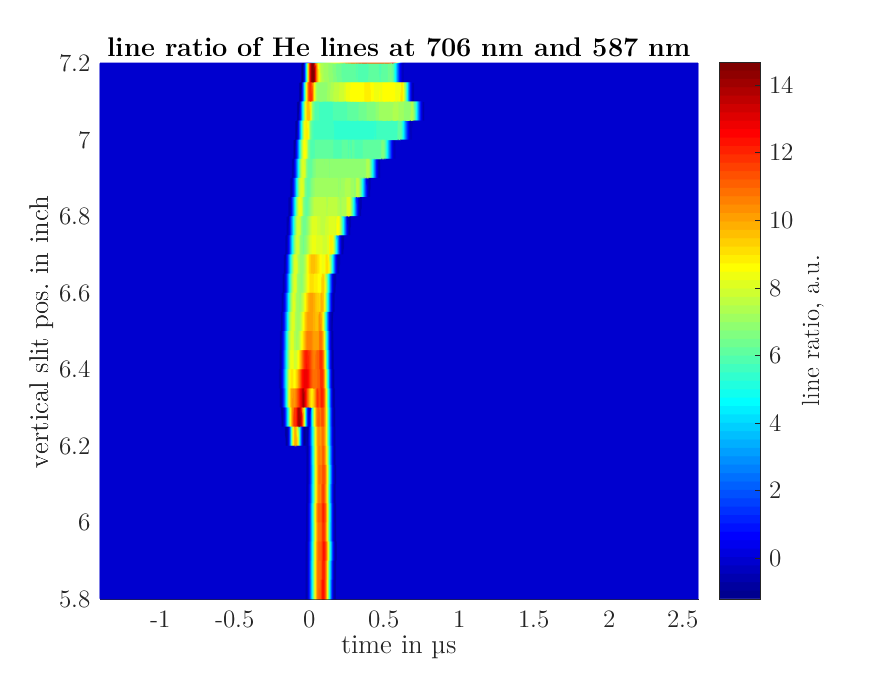
\includegraphics[width=\textwidth]{figures/results/lineratios/square/lineratio706}
						\vspace{-0.5cm}\caption{}
						\label{img:ratio7065}
					\end{subfigure}
					
					\begin{subfigure}[t]{0.48\textwidth}
						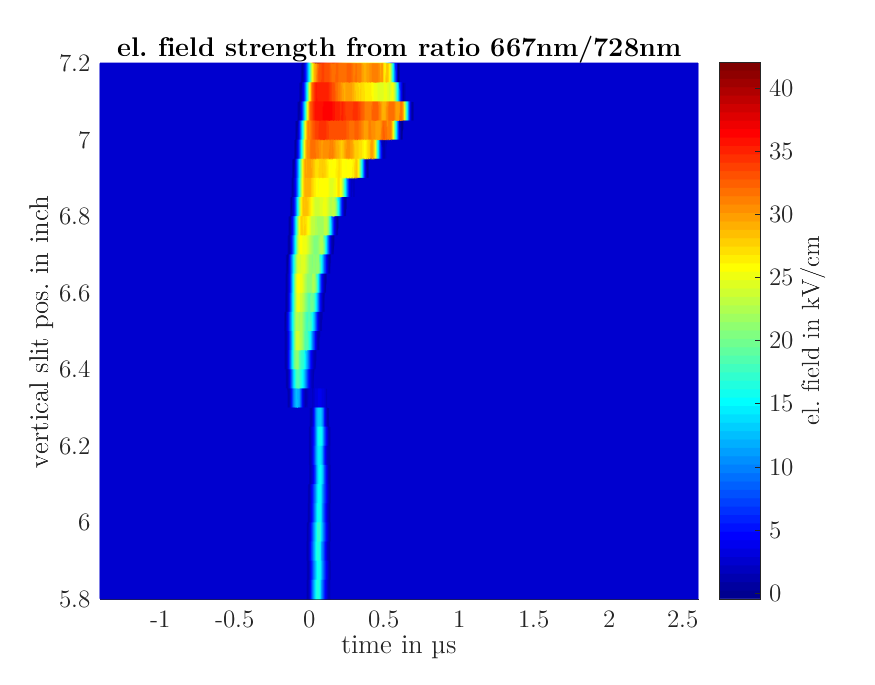
\includegraphics[width=\textwidth]{figures/results/lineratios/square/elfield667}
						\vspace{-0.5cm}\caption{}
						\label{img:elfield667}
					\end{subfigure}
					\hfill
					\begin{subfigure}[t]{0.48\textwidth}
						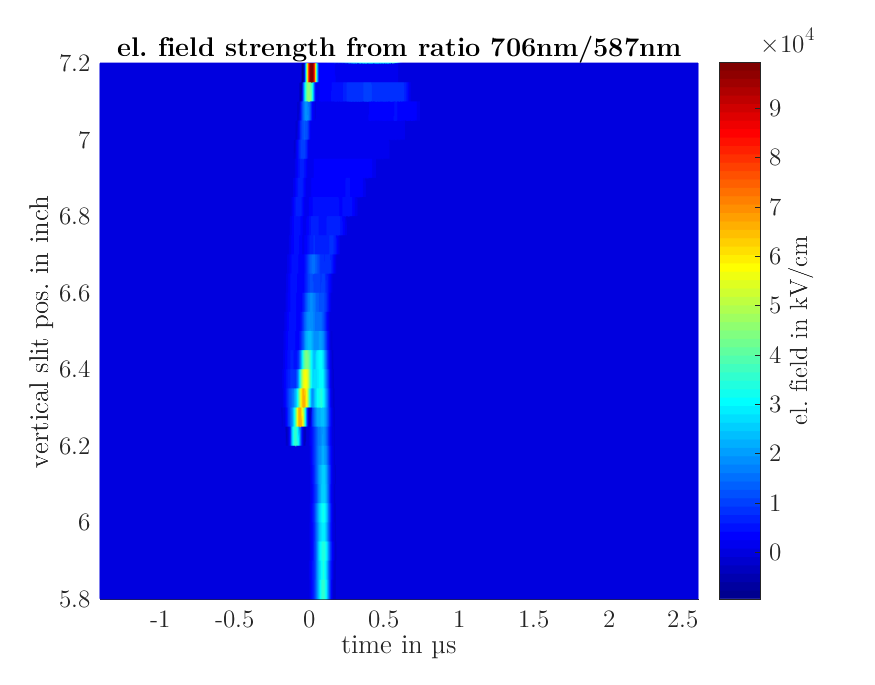
\includegraphics[width=\textwidth]{figures/results/lineratios/square/elfield706}
						\vspace{-0.5cm}\caption{}
						\label{img:elfield7065}
					\end{subfigure}
					
					\caption{\fett{(a):} Line ratio from the division of the intensity values of the emission at $\unit[667.96]{nm}$ and $\unit[728.31]{nm}$. \fett{(b):} Line ratio of $\unit[706.66]{nm}$/$\unit[587.65]{nm}$. \fett{(c):} \fett{(d):} }
				\end{figure}
				
		\twocolumn
		
		\subsection{Stark spectroscopy}

	\section{Conclusion}
		
	\section{Acknowledgments}
		
	\subsection{References}

		\bibliography{all.bib}
		\bibliographystyle{unsrt}

	\section{Appendix}


\end{document}